\chapter{Router}

The primary function of a router is: Determine the best path to send packets and Forward packets toward their destination.

\section{Packet-Forwarding Mechanisms}

\begin{itemize}
\item \textbf{Process switching:} Process switching starts finding a path every time a packet arrives, even if the destination is the same for a stream of packets. This mechanism is slow and old-fashioned.

\item \textbf{Fast switching:} The flow information for the packet is also stored in the \emph{fast-switching cache}. If another packet going to the same destination arrives on an interface, the next-hop information in the cache is reused without CPU intervention.

\item \textbf{Cisco Express Forwarding (CEF):} CEF builds a Forwarding Information Base (FIB), and an adjacency table, then stores them in the data plane. The FIB contains precomputed reverse lookups, next-hop information for routes including the interface, and Layer 2 information. Therefore, when a network has converged, the FIB and adjacency tables contain all the information a router would have to consider when forwarding a packet. This enables forwarding of packets to occur at the data plane without consulting the control plane.
\end{itemize}

\section{Router Switching Function}

The router performs the following three major steps (Figure \ref{SwitchingFunc}):

\begin{figure}[hbtp]
\caption{Encapsulating and De-encapsulating packets}\label{SwitchingFunc}
\centering
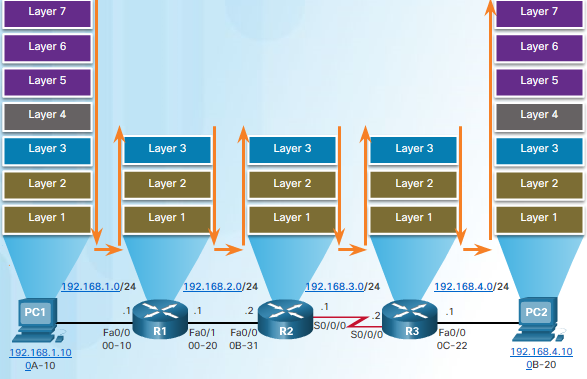
\includegraphics[scale=0.7]{pictures/SwitchingFunc.PNG}
\end{figure}


\begin{enumerate}
\item De-encapsulates the Layer 2 frame header and trailer to expose the Layer 3 packet.

\item Examines the destination IP address of the IP packet to find the best path in the routing table.

\item If the router finds a path to the destination, it encapsulates the Layer 3 packet into a new Layer 2 frame and forwards the frame out the exit interface. MAC addresses are only required on Ethernet multiaccess networks. A serial link is a point-to-point connection and uses a different Layer 2 frame that does not require the use of a MAC address. Because there are no MAC addresses on serial interfaces, a router sets the data link destination address to an equivalent of a broadcast.
\end{enumerate}

\section{Path determination}

A metric is the quantitative value used to measure the distance to a given network. The best path to a network is the path with the lowest metric. The following lists some dynamic protocols and the metrics they use:

\begin{itemize}
\item RIP -- hop count
\item OSPF -- bandwidth
\item EIGRP -- Bandwidth, delay, load, reliability
\end{itemize}

When a router has two or more paths to a destination with equal cost metrics, then the router forwards the packets using both paths equally. This is called equal cost \textbf{load balancing}. The routing table contains the single destination network but has multiple exit interfaces, one for each equal cost path. Only \emph{EIGRP} supports \emph{unequal cost load balancing}.\\

A router uses what is known as the \textbf{administrative distance (AD)} to determine the route to install into the IP routing table. The AD represents the trustworthiness of the route; the lower the AD, the more trustworthy the route source. For example, when a router has the choice of a static route (AD = 1) and an EIGRP route (AD = 90), the static route takes precedence. The following list shows the AD value of common routes:

\begin{itemize}
\item Connected interface = 0
\item Static route = 1
\item BGP = 20
\item Internal EIGRP = 90
\item OSPF = 110
\item RIP = 120
\item External EIGRP = 170
\item Internal BGP = 200
\end{itemize}